\documentclass[a4paper,12pt]{article}

\usepackage{graphicx} % Required for inserting images
\usepackage{amsmath,amssymb,amsfonts}
\usepackage{subcaption}
% Use Times New Roman font
\usepackage{times}
\usepackage[a4paper, top=1in, bottom=0.8in, left=1.1in, right=0.8in]{geometry}
\usepackage{float}
\usepackage{listings}
\usepackage{xcolor} % For customizing code colors
\setlength{\parindent}{0pt}
\usepackage{titlesec} % Add this to your preamble
\titleformat{\section}
{\normalfont\large\bfseries}{\thesection}{1em}{}
% Set spacing for sections
\titlespacing*{\section}
{0pt}  % Left spacing
{0ex} % Space before (adjust this value)
{0cm}  % Space after (adjust this value)
\begin{document}
	\section{Experiment No. 6}
	
	
	\section{Experiment Title }
	Design and Analyze 2 Input XOR and XNOR Gates Using 1Finger MOS on
	MICROWIND 3.0
	\section{Objective}
	The main objectives of this report are:
	\begin{itemize}
		\item To design and analyze XOR and XNOR gates using CMOS inverters.
		\item To compare the performance of XOR and XNOR gates in terms of output voltage levels and switching characteristics.
		\item To verify the logical behavior of the XOR and XNOR gates using truth tables.
		\item To simulate the gate designs using MICROWIND 3.0 and understand the impact of circuit configurations on output behavior.
	\end{itemize}
	
	\section{Theory}
	\subsection{CMOS XOR Gate}
	A 2-input CMOS XOR gate is constructed using both pMOS and nMOS transistors in a configuration that performs the exclusive OR function. The output is high (logic '1') only when the inputs \( A \) and \( B \) are different, i.e., when one is logic '1' and the other is logic '0'. If both inputs are the same (either logic '0' or logic '1'), the output is low (logic '0'). The logic function of the 2-input CMOS XOR gate can be expressed as:
	
	\[
	Y = A \oplus B = (A \cdot \overline{B}) + (\overline{A} \cdot B)
	\]
	
	where:
	- \( A \) and \( B \) are the inputs, and
	- \( Y \) is the output of the XOR gate.
	
	\begin{figure}[H]
		\centering
			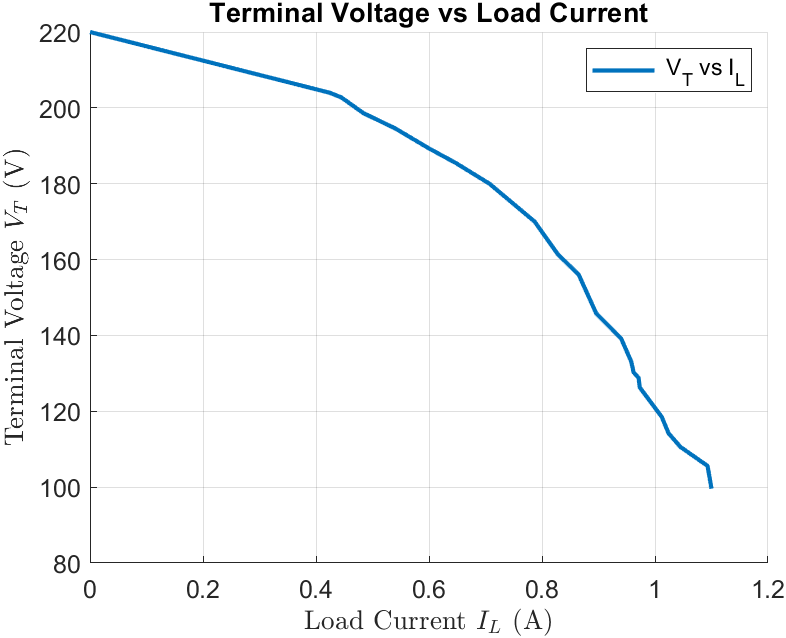
\includegraphics[width=0.40\linewidth]{"D:/DOWNLOAD 2024 V2/LATEX FILE/EEE_2214/EXP06_EEE2214/Images/1.1"}
		\caption{CMOS XOR-Gate}
		\label{fig:xor_gate}
	\end{figure}
	But in CMOS implementation,we use 
		\[
	Y = \overline{\overline{A \oplus B}} = (A \cdot B) + (\overline{A} \cdot \overline{B})
	\]
	The truth table for a 2-input XOR gate is shown below:
	
	\begin{table}[H]
		\centering
		\caption{Truth Table for 2-Input CMOS XOR Gate}
		\begin{tabular}{|c|c|c|}
			\hline
			\textbf{A} & \textbf{B} & \textbf{Y (XOR Output)} \\ \hline
			0          & 0          & 0                       \\ \hline
			0          & 1          & 1                       \\ \hline
			1          & 0          & 1                       \\ \hline
			1          & 1          & 0                       \\ \hline
		\end{tabular}
		\label{tab:xor_gate}
	\end{table}
	
	\subsection{CMOS XNOR Gate}
	A 2-input CMOS XNOR gate is constructed similarly to the XOR gate, but with an additional inverter at the output. The output is high (logic '1') when both inputs \( A \) and \( B \) are the same, and low (logic '0') when they are different. The logic function of the 2-input CMOS XNOR gate can be expressed as:
	
	\[
	Y = \overline{A \oplus B} = (A \cdot B) + (\overline{A} \cdot \overline{B})
	\]
	
	where:
	- \( A \) and \( B \) are the inputs, and
	- \( Y \) is the output of the XNOR gate.
	
	\begin{figure}[H]
		\centering
		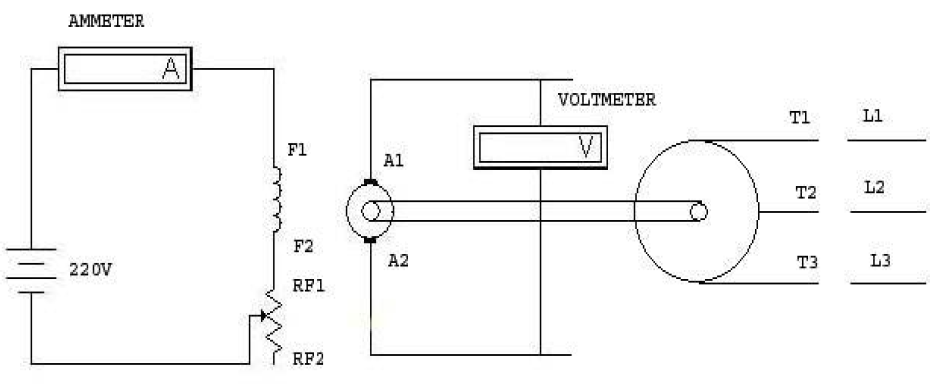
\includegraphics[width=0.39\linewidth]{"D:/DOWNLOAD 2024 V2/LATEX FILE/EEE_2214/EXP06_EEE2214/Images/2.1"}
		\caption{CMOS XNOR-Gate}
		\label{fig:xnor_gate}
	\end{figure}
	But in CMOS implementation,we use 
		\[
	Y = \overline{\overline{\overline{A \oplus B}}} = (A \cdot \overline{B}) + (\overline{A} \cdot B)
	\]
	
	The truth table for a 2-input XNOR gate is shown below:
	
	\begin{table}[H]
		\centering
		\caption{Truth Table for 2-Input CMOS XNOR Gate}
		\begin{tabular}{|c|c|c|}
			\hline
			\textbf{A} & \textbf{B} & \textbf{Y (XNOR Output)} \\ \hline
			0          & 0          & 1                        \\ \hline
			0          & 1          & 0                        \\ \hline
			1          & 0          & 0                        \\ \hline
			1          & 1          & 1                        \\ \hline
		\end{tabular}
		\label{tab:xnor_gate}
	\end{table}
	
	\newpage
	\section{Schematic Layout }
	
		\subsection{XOR Gate using 1 Finger MOS}
	\begin{figure}[H]
		\centering
		\includegraphics[width=0.7\linewidth]{"D:/DOWNLOAD 2024 V2/LATEX FILE/EEE_2214/EXP06_EEE2214/Images/1"}
		\caption{Design layout of XOR-Gate using 1 Finger MOS}
		\label{fig:1}
	\end{figure}
		\subsection{XNOR Gate using 1 Finger MOS}
	\begin{figure}[H]
		\centering
		\includegraphics[width=0.7\linewidth]{"D:/DOWNLOAD 2024 V2/LATEX FILE/EEE_2214/EXP06_EEE2214/Images/3"}
		\caption{Design layout of XNOR-Gate using 1 Finger MOS}
		\label{fig:1}
	\end{figure}
	
	\section{Specification}
		\begin{table}[H]
		\centering
		\caption{MOSFET Dimensions for nMOS and pMOS Transistors}
		\label{tab:MOSFET_dimensions}
		\begin{tabular}{|c|c|c|c|c|}
			\hline
			\textbf{MOS} & \textbf{\begin{tabular}[c]{@{}c@{}}Width\\ ($\mu m$)\end{tabular}} & \textbf{\begin{tabular}[c]{@{}c@{}}Length\\ ($\mu m$)\end{tabular}} & \textbf{\begin{tabular}[c]{@{}c@{}}Width\\ ($\lambda$)\end{tabular}} & \textbf{\begin{tabular}[c]{@{}c@{}}Length\\ ($\lambda$)\end{tabular}} \\ \hline
			nMOS & 0.600 & 0.120 & 10 & 2 \\ \hline
			pMOS & 0.600 & 0.120 & 10 & 2 \\ \hline
		\end{tabular}
		
	\end{table}
	
	\begin{table}[H]
		\centering
		\caption{Parameters of Input Clock Signal for XOR-Gate and XNOR-Gate}
		% Sub-table (a)
		\begin{subtable}[t]{0.48\textwidth} % Adjusted width for each sub-table
			\centering
			\begin{tabular}{|c|c|c|}
				\hline
				\textbf{Parameter}          & \textbf{Value} & \textbf{Unit} \\ \hline
				High Level $(V)$            & 5.00           & $V$           \\ \hline
				Low Level $(V)$             & 0.00           & $V$           \\ \hline
				Time Low $(tl)$             & 0.225          & $ns$          \\ \hline
				Rise Time $(tr)$            & 0.001          & $ns$          \\ \hline
				Time High $(th)$            & 0.225          & $ns$          \\ \hline
				Fall Time $(tf)$            & 0.001          & $ns$          \\ \hline
			\end{tabular}
			\caption{Input clock signal of A} % Sub-table (a) caption
		\end{subtable}
		\hfil
		% Sub-table (b)
		\begin{subtable}[t]{0.48\textwidth} % Adjusted width for each sub-table
			\centering
			\begin{tabular}{|c|c|c|}
				\hline
				\textbf{Parameter}          & \textbf{Value} & \textbf{Unit} \\ \hline
				High Level $(V)$            & 5.00           & $V$           \\ \hline
				Low Level $(V)$             & 0.00           & $V$           \\ \hline
				Time Low $(tl)$             & 0.452         & $ns$          \\ \hline
				Rise Time $(tr)$            & 0.001          & $ns$          \\ \hline
				Time High $(th)$            & 0.452          & $ns$          \\ \hline
				Fall Time $(tf)$            & 0.001          & $ns$          \\ \hline
			\end{tabular}
			\caption{Input clock signal of B} % Sub-table (b) caption
		\end{subtable}
	\end{table}
	
	\begin{table}[H]
		\centering
		\caption{Parameters of Input Clock Signal for XOR-Gate and XNOR-Gate}
		% Sub-table (a)
		\begin{subtable}[t]{0.48\textwidth} % Adjusted width for each sub-table
			\centering
			\begin{tabular}{|c|c|c|}
				\hline
				\textbf{Parameter}          & \textbf{Value} & \textbf{Unit} \\ \hline
				High Level $(V)$            & 0.00           & $V$           \\ \hline
				Low Level $(V)$             & 5.00           & $V$           \\ \hline
				Time Low $(tl)$             & 0.225          & $ns$          \\ \hline
				Rise Time $(tr)$            & 0.001          & $ns$          \\ \hline
				Time High $(th)$            & 0.225          & $ns$          \\ \hline
				Fall Time $(tf)$            & 0.001          & $ns$          \\ \hline
			\end{tabular}
			\vspace{0.2cm}
			\caption{Input clock signal of $\bar{A}$} % Sub-table (a) caption
		\end{subtable}
		\hfil
		% Sub-table (b)
		\begin{subtable}[t]{0.48\textwidth} % Adjusted width for each sub-table
			\centering
			\begin{tabular}{|c|c|c|}
				\hline
				\textbf{Parameter}          & \textbf{Value} & \textbf{Unit} \\ \hline
				High Level $(V)$            & 0.00           & $V$           \\ \hline
				Low Level $(V)$             & 5.00           & $V$           \\ \hline
				Time Low $(tl)$             & 0.452        & $ns$          \\ \hline
				Rise Time $(tr)$            & 0.001          & $ns$          \\ \hline
				Time High $(th)$            & 0.452          & $ns$          \\ \hline
				Fall Time $(tf)$            & 0.001          & $ns$          \\ \hline
			\end{tabular}
				\vspace{0.2cm}
			\caption{Input clock signal of $\bar{B}$} % Sub-table (a)
		\end{subtable}
		
		
		
	\end{table}
	\begin{table}[H]
		\centering
		\caption{Parameters for Vdd+ and Vss- }
		\begin{tabular}{|c|c|c|}
			\hline
			\textbf{Parameter} & \textbf{Value} & \textbf{Unit} \\ \hline
			Vdd+               & 5.00           & $V $            \\ \hline
			Vss-               & 0.00           & $V$             \\ \hline
		\end{tabular}
		
	\end{table}
	
	\newpage
	\section{Output Waveshape }
	\subsection{CMOS XOR Gate}
	\begin{figure}[H]
		\centering
		\includegraphics[width=1\linewidth, height=.39\textheight]{"D:/DOWNLOAD 2024 V2/LATEX FILE/EEE_2214/EXP06_EEE2214/Images/2"}
		\caption{Output Waveshape of XOR-Gate using 1 Finger MOS}
		\label{fig:1}
	\end{figure}
	\subsection{CMOS XNOR Gate}
	\begin{figure}[H]
		\centering
		\includegraphics[width=1\linewidth, height=.39\textheight]{"D:/DOWNLOAD 2024 V2/LATEX FILE/EEE_2214/EXP06_EEE2214/Images/4"}
		\caption{Output Waveshape of XNOR-Gate using 1 Finger MOS}
		\label{fig:1}
	\end{figure}
	\section{Discussion}
The characteristics of  CMOS XOR and XNOR gates were analyzed based on the input signals \(A\) and \(B\) and the corresponding output signal \(Y\). It was observed that the output of the XOR gate was the complement of the output of the XNOR gate for all input combinations, indicating that they are logical inverses of each other. The truth tables confirmed that when the XOR gate output is logic high, the XNOR gate output is logic low, and vice versa.\\
During testing, the XOR gate exhibited some voltage fluctuations during state transitions, which were also present in the XNOR gate. This behavior in the XOR and XNOR gate could be attributed to the charge and discharge dynamics of its pMOS and nMOS transistors during switching. Despite these fluctuations, both gates adhered to the expected logical behavior as outlined in the truth table.
	
	
\end{document}